\vspace{-5.5mm}
{\small
\begin{itemize}
\item Expected value: $E = \sum_{i=1}^{n} P_i \cdot i$
\item Variance: $V(x) = E(x^2) - \{E(x)\}^2$
\item To get two consecutive heads, what is the expected number of tosses?
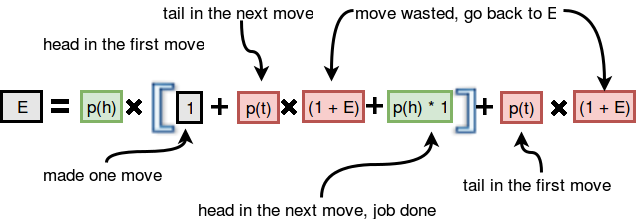
\includegraphics[width=\linewidth]{images/expected_value_1.png}
\item To get $n$ heads, what is the expected number of tosses? Let’s define: to get $n$ heads, we need to toss $E(n)$ times. Now — I can get a head; I need to toss $E(n-1)$ more times, or if I get a tail; I need to toss $E(n)$ times. So, the recurrence is: $E(n) = 0.5 \cdot (1 + E(n-1)) + 0.5 \cdot (1 + E(n))$
% 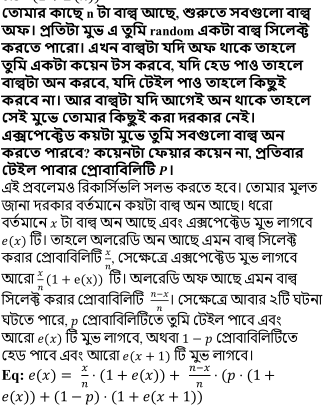
\includegraphics[width=\linewidth]{images/expected_value_2.png}
\item {
    You have $n$ bulbs, all of which are initially off. In each move, you randomly select one bulb. If the selected bulb is \textbf{off}, you toss a coin:
    \begin{itemize}
        \item If you get head, you turn it on.
        \item If you get tail, you do nothing.
    \end{itemize}

    If the bulb is already \textbf{on}, you skip that move (nothing happens).

    \par % Use par for a clean paragraph break
    Now, what is the expected number of moves required to turn all bulbs on?

    The coin is not fair — the probability of getting tail is $p$.
    This problem can also be solved recursively.

    \par
    Let's assume at some moment, $x$ bulbs are already on, and the expected number of moves needed from here is $e(x)$.

    The probability of picking an already on bulb is $\frac{x}{n}$.
    In that case, the expected number of moves is $\frac{x}{n} \times (1 + e(x))$.

    The probability of picking an off bulb is $\frac{n-x}{n}$.

    \par
    Now two things can happen:
    \begin{itemize}
        \item With probability $p$, you get tail, so you stay at the same state ($e(x)$ more moves).
        \item With probability $(1-p)$, you get head, so one more bulb turns on ($e(x+1)$ moves from there).
    \end{itemize}

    \par
    So, the recurrence relation is:
    \begin{align*}
    e(x) &= \frac{x}{n} (1 + e(x)) + \\
         & \quad \frac{n-x}{n} \big( p(1 + e(x)) + (1-p)(1 + e(x+1)) \big)
    \end{align*}
}
\end{itemize}
}
